\chapter{Creating Charts}
\section{Bar Chart}
    \begin{figure}[h!]
    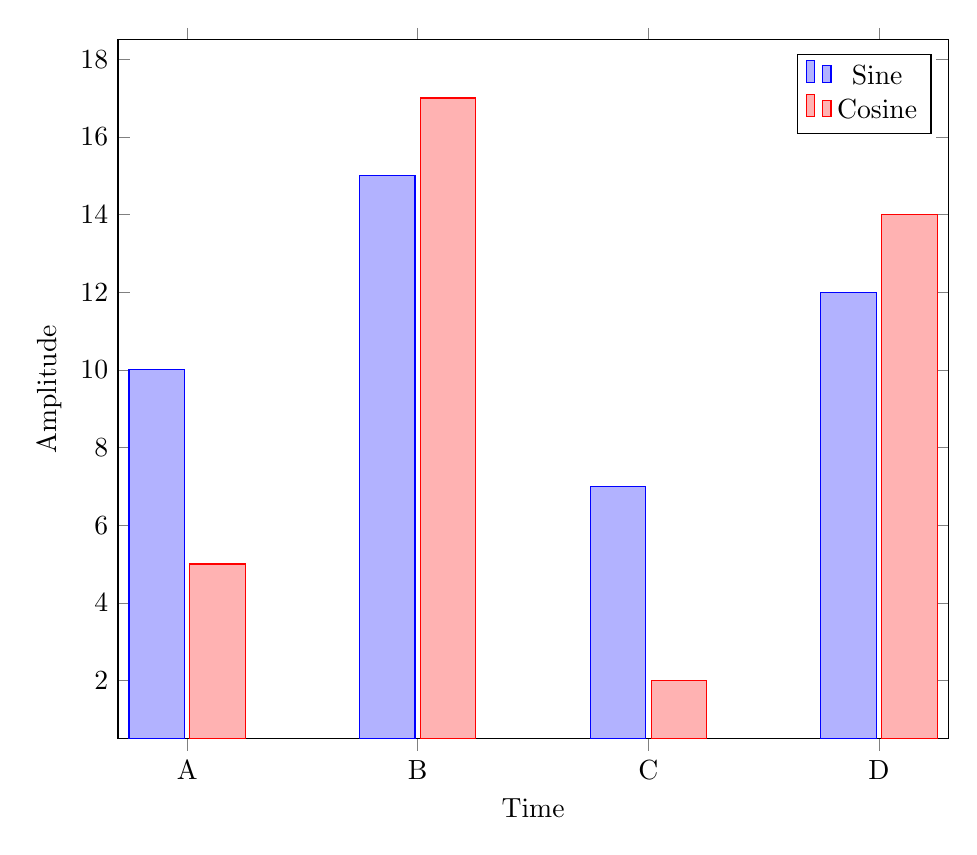
\begin{tikzpicture}
        \begin{axis}[
            width = 1\textwidth,
            xtick = data,
            ybar,
            bar width =20pt,
            enlarge x limits=0.1,
            ylabel={Amplitude},
            xlabel={Time},
            symbolic x coords={A, B, C, D},
            ]
            \addplot coordinates {(A,10) (B,15) (C,7) (D,12)};
            \addplot coordinates {(A,5) (B,17) (C,2) (D,14)};

            \legend{Sine,Cosine}
        \end{axis}
    \end{tikzpicture}
    \caption{Example Bar Chart}
    \label{fig:barchart}
\end{figure}


\newpage
\section{Gantt Chart}

\begin{figure}[h!]
    \hspace*{-5em}
    \begin{ganttchart}[
        x unit=30pt,
        y unit chart=30pt,
        time slot format=isodate-yearmonth,
        time slot unit=month,
        title height=1,
        bar/.append style={fill=blue!40},
        bar height=0.7
        ]{2024-04}{2025-03}
        \gantttitlecalendar{year} \\
        \gantttitlecalendar{month} \\
        \ganttbar{Req Analysis}{2024-04}{2024-05} \\
        \ganttbar{Feasibility Study}{2024-04}{2024-05} \\
        \ganttbar{Software Design}{2024-05}{2024-06} \\
        \ganttbar{Implementation}{2024-06}{2025-01} \\
        \ganttbar{Testing}{2025-01}{2025-02} \\
        \ganttbar{Research}{2024-04}{2025-01}\\
        \ganttbar{Documentation}{2024-04}{2025-03}\\
    \end{ganttchart}
    \caption{Gantt Chart}
\end{figure}
